\documentclass[journal,twocolumn,12pt]{ieeesyscoin}
\usepackage{cite}
\usepackage{amsmath,amssymb,amsfonts}
\usepackage{algorithmic}
\usepackage{enumitem}
\usepackage{caption}
\usepackage{xcolor}
\usepackage{graphicx}
\usepackage{textcomp}
\usepackage{multirow}
\usepackage{lipsum}
\usepackage{makecell}
\usepackage[switch]{lineno}
\def\BibTeX{{\rm B\kern-.05em{\sc i\kern-.025em b}\kern-.08em
    T\kern-.1667em\lower.7ex\hbox{E}\kern-.125emX}}
\begin{document}

\history{}

\title{\centering An Analytical and Empirical Survey of Impermanent Loss}
\author{\centering \uppercase{Ian C. Moore, PhD}\authorrefmark{1},and
\uppercase{Jagdeep Sidhu, MSc}\authorrefmark{2}}

\address[1]{\centering  Syscoin Researcher, Syscoin Platform (e-mail: imoore@syscoin.org)}
\address[2]{\centering Syscoin Lead Developer, (e-mail: sidhujag@syscoin.org)}
\tfootnote{}

\markboth
{Moore \headeretal: An Analytical and Empirical Survey of Impermanent Loss}
{Moore \headeretal: An Analytical and Empirical Survey of Impermanent Loss}

\corresp{}

\begin{abstract}

Automated market maker (AMM) protocols have played a key role in decentralized finance (DeFi) since Uniswap successfully launched the first constant product market maker in 2018. The popularity of these protocols have since increased to a global market size now measured in billions of US dollars. With this increased demand, there is a need to mitigate losses and maximize yield on these new platforms. In this discussion, we conduct an analytical and empirical survey on the risk profile of these liquidity providers for Uniswap v2, which is commonly known as Impermanent Loss. 

\end{abstract}

\begin{keywords}
Impermanent Loss, Liquidity Pool Management, Decentralized Finance, DAOSYS
\end{keywords}

\titlepgskip=-15pt

\maketitle

\section{Introduction}
\label{sec:introduction}

An automated market maker (AMM) protocol is the mechanism used by decentralized exchanges (DEXs) and was first introduced by Uniswap, which was launched on the Ethereum mainnet in November 2018. These DEXs consist of liquidity pools (LPs) represented by various trading pairs (eg. ETH/USDC, ETH/WBTC, etc.) acting as the AMM. Trading activity within these LPs are governed via smart contract through the \textit{constant product trading formula}:

\begin{equation}\label{eqn:cpt}
xy = k,
\end{equation}
where $x$ represents the number of tokens for one asset, $y$ represents the number of tokens for the other, and $k$ is a constant, which helps maintain asset price.

When a user places a trade on the DEX, they will typically pay a 0.3\% fee which is added to the LP. These cumulated fees are divided proportionally and paid out to all the providers of that particular LP as a yield payment. These collected yields from trading fees provide incentive for liquidity providers to invest in these LPs. This allows LP providers, who would otherwise be regular \textit{hodlers}, to earn additional yield from their assets.

When providers add funds to an LP, the apportioned value to each asset is split 1:1 in USD terms. For instance, say Ethereum is priced at \$1,500 per ETH and a provider wants to invest into an ETH/USDC LP, then the provider would have to invest 1 ETH along with an additional \$1,500 USDC for a total initial investment value of \$3,000 USD. The issue that can arise from investing into these LPs is that there are instances where the USD value of a liquidity provider's stake can decrease (ie, when compared against regular hodling) despite receiving yields from trading fees. This loss is known as Impermant Loss (IL), which was first termed by Pintail in \cite{Pin19a, Pin19b}. Many have argued that this term is a bit of a misnormer as the term \textit{impermanent} could create the expectation that losses are subject to a guaranteed reversal, which is not always the case. In 2020, Pintail later updated the term in his original articles to Divergent Loss. However, between that time, the former term had already been adopted by the decentralized finance (DeFi) community. Since this effect is more broadly known as Impermanent Loss, we will be using it for the duration of this discussion.

The motivation for this analysis came out of the need to mitigate losses and maximize yield for a new smart DAO (ie, DAOSYS) that we are setting up on Syscoin's soon to be launched L2 network which is expected to go live mid-to-late 2023 \cite{Doge22}. In this article we provide an analytical and empirical a survey of IL and analytically show that expected impermanent loss is exactly computable and provide simulations to support the analysis. In summary, we provide a general easy-to-follow general guideline for LP managers to best manage their DEXs.

\section{Analytical Survey}

\subsection{Expected Impermanent Loss}
\label{sec:exp_impermanent_loss}

Impermanent (divergence) Loss is defined as:
\begin{equation}\label{eqn:imp_loss}
IL = \frac{V - V_{H}}{V_{H}},
\end{equation}
where $V$ is the initial value of the portfolio holding, derived as:
\begin{equation}\label{eqn:initial_lp_value}
V = 2L\sqrt{P_{0}\alpha},
\end{equation}
where $L$ is the liquidity, $P_{0}$ is the initial price, $\alpha$ is the price ratio (i.e., $\frac{p_{0}}{p_{f}}$), $V_{H}$ is the held portfolio value, and is derived by the following:
\begin{equation}\label{eqn:held_lp_value}
V_{H} = 2L\sqrt{P_{0} (1+\alpha)}.
\end{equation}
Derivations for (\ref{eqn:initial_lp_value}) and (\ref{eqn:held_lp_value}) are relatively straight forward and can be found in \cite{Aig21,Pet21}, and when applied to the definition of IL in (\ref{eqn:imp_loss}) we get:
\begin{equation}\label{eqn:imp_loss_derv}
IL = \frac{2\sqrt{\alpha}}{1+\sqrt{\alpha}} - 1.
\end{equation}

Eq. (\ref{eqn:imp_loss_derv}) has been used quite extensively \cite{Pin19a,Pin19b,Aig21,Pet21} as it provides a way of retrospectively quantifying LP risk expressed in terms of price ratio, $\alpha$. However, it provides no predictive insight as there is no consideration for historical stochastic price behaviour of a pair of assets. To provide this, we assume that LP price assets behave as a Geometric Brownian Motion (GBM) process, as first discussed in \cite{Gui21}. Using GBM to describe price behaviour has been widely adopted in the financial community; for more context, see Appendix \ref{sec:gbm}. When representing IL stochastically, its expectation can be derived as:

\begin{equation}\label{eqn:exp_imp_loss}
  E\{IL\} = \frac{e^{-\frac{\sigma^2 t}{8}}}{\cosh (\frac{\mu t}{2})} - 1.
\end{equation}
Eq. (\ref{eqn:exp_imp_loss}) provides some predictive insight on the performance of an LP, given an asset's historical price drift, $\mu$, and volatility, $\sigma$; see Fig. \ref{fig:exp_imp_loss}. This expression for the expectation of IL was first found in \cite{Gui21}, but with no derivation or explanation on how it was derived, however \cite{Dan22} provides a good elaboration on it's derivation, but with missing steps. For a full analytical derivation of (\ref{eqn:exp_imp_loss}), where the remaining steps are provided, see Appendix \ref{sec:exp_imp_loss_derv}.

\begin{figure}[h!]
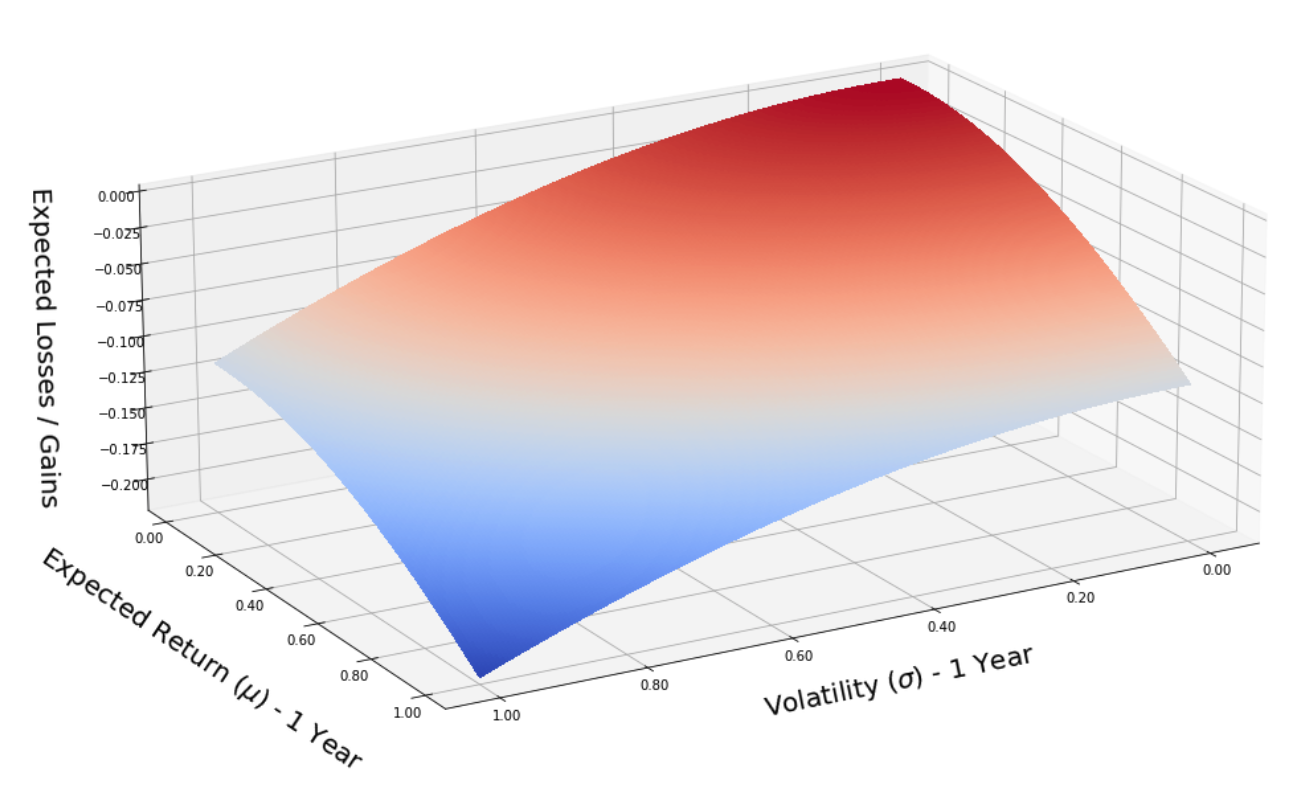
\includegraphics[width=3in]{img/imp_loss.png}
\caption{Expected impermanent loss for first year (ie, t = 1) using (\ref{eqn:exp_imp_loss}); expected IL drops with increasing drift and volatility.} 
\label{fig:exp_imp_loss}
\end{figure}

\subsection{Expected Portfolio Values}
\label{sec:exp_portfolio_value}
If we consider our assumption that price assets behave as a GBM process, then a portfolio of held assets from (\ref{eqn:held_lp_value}) is determined by:

\begin{equation}\label{eqn:held_portfolio}
  V_{H,t} = L \sqrt{P_{0}}(1 + e^{(\mu - \frac{\sigma^2}{2})t + \sigma W_{t} }),
\end{equation}
with an expectation of:
\begin{equation}\label{eqn:exp_held_portfolio}
  E\{V_{H}\} = 2 L \sqrt{P_{0}} (1 + e^{\mu t}).
\end{equation}
Likewise, our outside portfolio value of (\ref{eqn:initial_lp_value}) becomes:
\begin{equation}\label{eqn:portfolio_outside}
  V_{t} = 2L \sqrt{P_{0}} e^{(\frac{\mu}{2} - \frac{\sigma^2}{4})t } e^{   \frac{1}{2}\sigma W_{t}}, 
\end{equation}
with an expectation of:
\begin{equation}\label{eqn:exp_portfolio_outside}
  E\{V\} = 2 L \sqrt{P_{0}}  e^{(\frac{\mu t}{2} - \frac{\sigma^2 t}{8})}.
\end{equation}
For the derivation of the expectations in (\ref{eqn:exp_held_portfolio}) and (\ref{eqn:exp_portfolio_outside}), see Appendix C.

\subsection{Expected Returns with Compounding Fees}
\label{sec:exp_lp_returns}
If we take the aggregation of individual deposits $a_{i}$ in the form of a geometric mean, this can be expressed by the following:

\begin{equation}\label{eqn:geo_mean}
  (\prod_{i=1}^{n}a_{i})^{\frac{1}{n}} = e^{\frac{1}{n}\sum_{i}^{n}\ln a_{i}}.
\end{equation}
For sake of brevity, we assume $\beta = \frac{1}{n}\sum_{i}^{n}\ln a_{i}$, hence the growth term becomes:
\begin{equation}\label{eqn:geo_mean}
  F_{t} = C_{0} e^{\beta t}
\end{equation}
where $\beta$ represents constant rate of growth and $C_{0}$ represents initial deposit. Hence, we consider (\ref{eqn:geo_mean}) to be a simple portfolio growth model. If we consider a dynamic variant of $C_{0}$ in the trading fees model of (\ref{eqn:geo_mean}), the expectation of (\ref{eqn:exp_portfolio_outside}) becomes:
\begin{equation}\label{eqn:exp_portfolio_outside_with_fees}
  E\{V\} = 2 L \sqrt{P_{0}}  e^{(\frac{\mu t}{2} - \frac{\sigma^2 t}{8})}e^{ \beta t}.
\end{equation}
If we consider the expected portfolio value with fee model in (\ref{eqn:exp_portfolio_outside_with_fees}), and the template outlined in Appendix C, the expected LP returns can be determined as follows:  
\begin{equation}\label{eqn:exp_returns_with_fees}
  E\{R\} = \frac{e^{-\frac{\sigma^2 t}{8} + z_{t}}}{\cosh (\frac{\mu t}{2})}.
\end{equation}
The term $e^{z_{t}}$ in (\ref{eqn:exp_returns_with_fees}), represents portfolio growth due to the accumulation of trading fees, where $z_{t}$ can be updated to consider various nuances in trading fee behaviour; see Fig. \ref{fig:imp_loss_compounding_fees}.

\begin{figure}[h!]
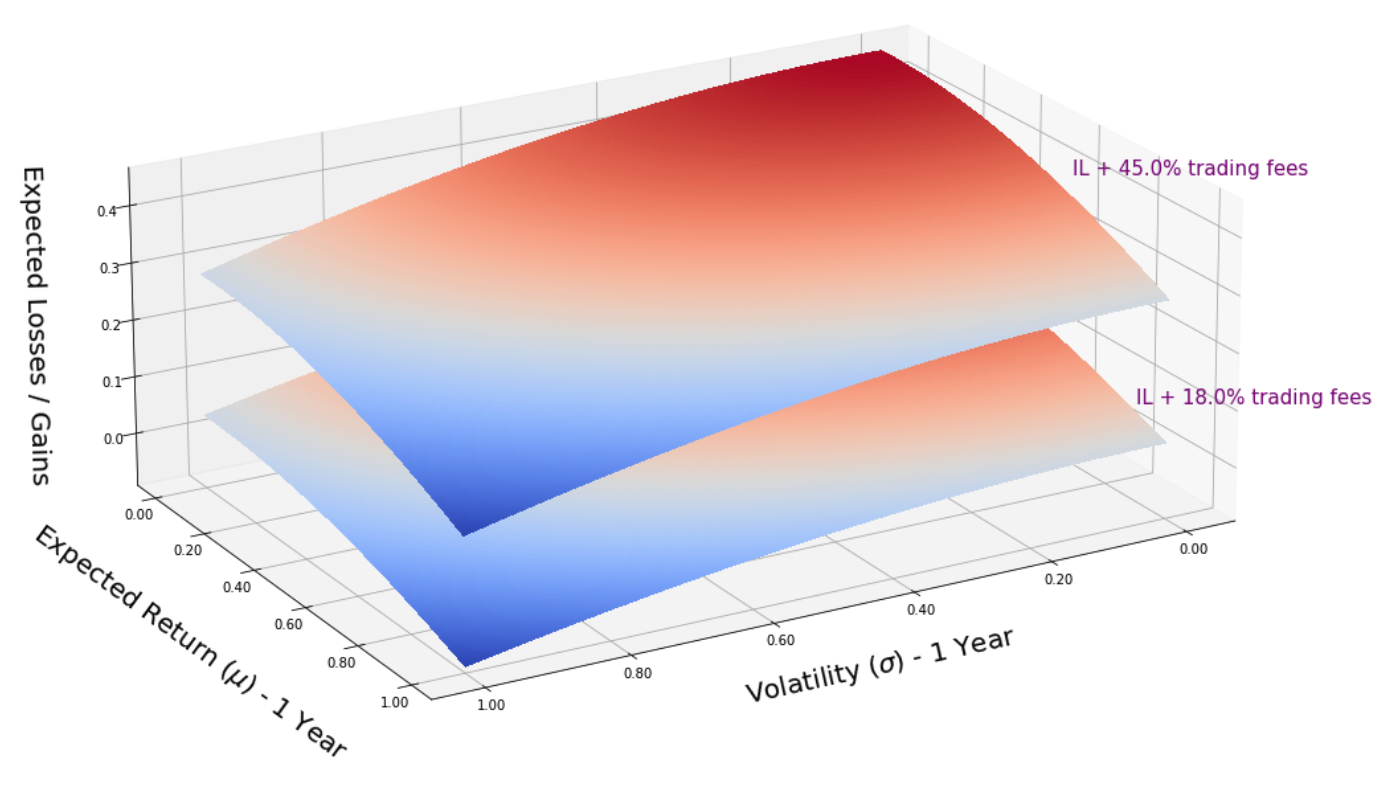
\includegraphics[width=3in]{img/imp_loss_compounding_fees.png}
\caption{Expected impermanent loss with compounding trading fees for first year (ie, t = 1)  using (\ref{eqn:exp_returns_with_fees}); increased trading activity results in a upwards shifting of the curve.}
\label{fig:imp_loss_compounding_fees}
\end{figure}

\section{DeFi Python Simulator}
\label{sec:python_simulator}

Despite popular perception, treasuries of Decentralized Autonomous Organizations (DAOs) tend to be centrally controlled and do not reflect the true ethos of cryptocurrency (i.e., \textit{not your keys, not your coins}). Syscoin is solving this problem via DAOSYS, which is a new smart DAO protocol technology for DeFi \cite{Doge22}, which will be launched sometime in 2023 on Syscoin's L2 Rollux platform.

To realize proper tokenomics design, it is highly inefficient to invest resources into development without first simulating the design to test specifications for various outcomes. This is what every DeFi project in the crypto space is not doing. This is why we are introducing an open source python package to simulate various sandboxed DeFi components of DAOSYS so that project engineers, managers and designers can pre-plan outcomes prior to investing valuable resources into development. 

With this tool, DAOSYS designers can utilize the plug and play components of our simulator to build tokenomics mockups for business planning purposes so that teams can come together and get collective consensus alongside potential users and investors. Not only is this tool applicable to DAOSYS, it can be used as a general purpose tool to simulate DEX activity for anyone wishing to setup their own LP and wish to stress test their ideas prior to development. This can be used as a powerful design tool to explore the limitations of a DeFi project idea prior to committing valuable resources on development costs (ie, Devs and Project Managers). Table \ref{table:simulator_components} highlights some key components of our DeFi simulator to provide potential users of the system a higher understanding of the package.

\begin{table}[h]
\centering
\begin{tabular}{ |l|l| } 
\hline
 \textbf{Simulator Component} & \textbf{Description} \\
\hline
\verb|BrownianModel|          & Generate Geometric Brownian motion   \\
					 &  (GBM) price simulation for a given $\mu$, $\sigma$, $t$,\\
					 &  and  \#  of steps; see Appendix \ref{sec:gbm} \\
\verb|SolveDeltas|          & Solve swap values $\Delta x_{k}$ and $\Delta y_{k}$ for a  \\
					&  given price change  $\Delta p_{k}$; see Appendix \ref{sec:lp_swap_deltas}\\ 
\verb|Liquidity|          & Maintains asset holdings $x_{k}$, $y_{k}$, $\Delta x_{k}$,  \\
				   &  $\Delta y_{k}$, liquidity value, price, and fee at time  \\ 
				   &  sample $k$ \\
\verb|LiquidityPoolUSD|          & Calculates USD LP values of various \\
						&	 forms, given $\{x_{k}\}_{0}^{N}$,  $\{y_{k}\}_{0}^{N}$, and  $\{p_{k}\}_{0}^{N}$; \\ 
					    &	see Figs. \ref{fig:price_sims} and \ref{fig:lp_vals} \\ 
\verb|EventSelectionModel|          & Generates random binomial process  \\ 
							& representing withdrawal and deposit events,   \\
							& where  Pr(deposit) = $p$, Pr(withdraw) = $p$-1  \\
							& and $p \in [0,1]$  \\
\verb|TokenDeltaModel|          & Generates deposit and withdrawals deltas\\ 
					     & $\Delta x_{k}$ and $\Delta y_{k}$ randomly sampled from a \\
					     & gamma distribution\\		
\verb|SimulateLiquidity|          & Simulates LP activity of swaps, deposits   \\
						  & and withdrawals given  \\
						  & \verb|TokenDeltaModel|,  \verb|Liquidity|   \\
						  & objects  and  pre-generated  GBM simulation \\ 
\verb|CalcLPFees|          & Calculate LP fees (0.3\% per swap) \\

\hline
\end{tabular}
\caption{Descriptions of DeFi python simulator components that was used to generate LP simulations}
\label{table:simulator_components}
\end{table}

We have a working beta version of the simulator which is available through Syscoin’s Github repository. This simulator is being built alongside DAOSYS, and we are using this to understand the ROI and design considerations for DAOSYS’s first usecase (ie, Masternode Yield Farming). Since the simulator is still in the beta stage, the setup is currently not realized to its full intention. However, a usable demo of this tool is available from Syscoin's Github repository for the community to begin using. For a mini python tutorial on how to use this tool, please refer to \cite{Moo22B, DAOSim22} for a series of example Jupyter notebooks.

The purpose of this tool is primarily for the design aspect of DAOSYS, and is still in its early stages of development. The next stages involve feeding the output of various mathematical models into the simulator framework and to use this tool to simulate other DeFi usecases. This allows us to test a roster of edge cases for building more robust systems. The final goal is to bring this system to a level of maturity so that it can be utilized in parallel with the contracts in real time. Hence, exposing DeFi to a scientific way of design, testing, and implementation.


\section{Numerical Simulations}
\label{sec:numerical_simulations}

In Section \ref{sec:exp_impermanent_loss} we provided the analytic approach to calculating expected IL in (\ref{eqn:exp_imp_loss}) and expect returns in (\ref{eqn:exp_returns_with_fees}). In this Section, we provide numerical outcomes using our Defi simulator outlined in Section \ref{sec:python_simulator} to support the analysis.

To simulate LP Activity using GBM price simulations, we implemented the following using the components described in Table \ref{table:simulator_components}: 
\begin{enumerate}
	\item Instantiate \verb|Liquidity| object to maintain LP state 
	\item Instantiate \verb|SimulateLiquidity| object to govern LP simulation events
	\item Generate GBM price sequence simulation, $\{p_{k}\}_{0}^{N}$, using \verb|BrownianModel|
	\item Using \verb|SimulateLiquidity| object, run LP simulation, for every time sample, $k$, do:
  \begin{enumerate}
    \item Solve swap deltas $\Delta x_{k}$ and $\Delta y_{k}$ using \verb|SolveDeltas| given $p_{k}$; see Appendix \ref{sec:lp_swap_deltas}
    \item Calculate swap fee, $r_{k}$
    \item Run \verb|EventSelectionModel| to determine deposit or withdrawal event with probability $Pr\{deposit\}$ = 0.55
    \item Using outcome of previous step, add or subtract liquidity from pool to simulate LP growth or decline
    \item Using \verb|Liquidity| object, update LP state 
  \end{enumerate}
  \item Repeat steps 1-4 \verb|n_path| times
	
\end{enumerate}
The python code for the above procedure is openly available through Syscoin's Github repository, which can be accessed via \cite{DAOSim23}. Using this stepwise process, we generate the numerical results which are presented in Tables \ref{table:sim_vs_theory1} and \ref{table:sim_vs_theory2} for various configurations of drift ($\mu$), volatility, ($\sigma$), and sample size ($N$). These numerical results for expected IL and returns are compared against the theoretical results using (\ref{eqn:exp_imp_loss}) and (\ref{eqn:exp_returns_with_fees}) respectively.

We also present simulated temporal LP outcomes from our DeFi simulator as shown in Figs. \ref{fig:price_sims}, \ref{fig:lp_vals}, and \ref{fig:lp_sims}. Each temporal sample represents the aggregate activity of one time interval which account for typical LP actions such as swaps, deposits and withdraws. It is well-studied that GBM processes are an effective tool to model asset price behavior; see Appendeix A. Thus, activity due to swaps are driven by a set of GBM price sequence paths presented in Fig. \ref{fig:price_sims}, and swap deltas $\Delta x$, $\Delta y$ are calculated using the non-linear set of equations presented in Appendix \ref{sec:lp_swap_deltas}. 

\begin{figure}[h!]
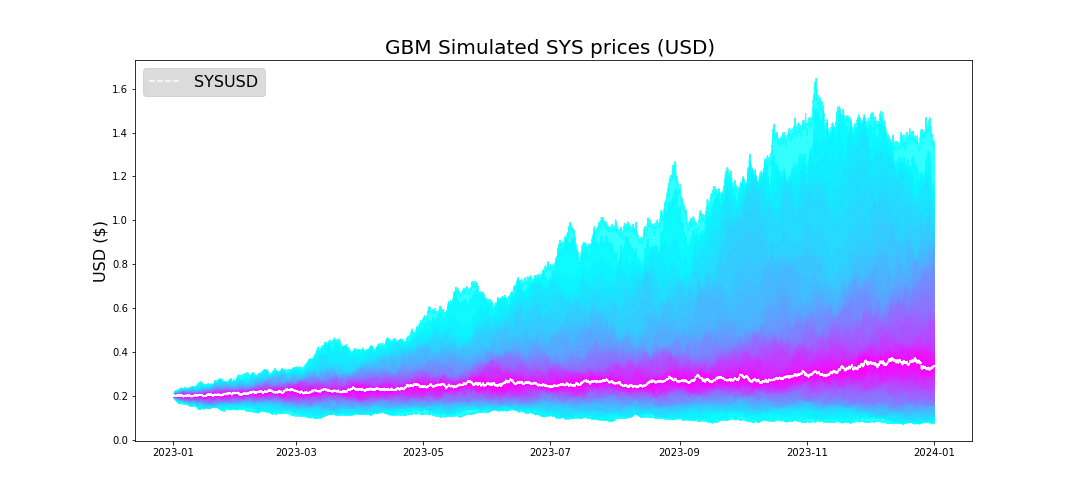
\includegraphics[width=3in]{img/price_simulations.png}
\caption{Set of simulated geometric Brownian motion (GBM) price sequence, $\{p_{k}\}_{0}^{N}$, paths where $\sigma = 0.5$ and $\mu = 0.4$ representing simulated SYSUSD prices; see Appendix A} 
\label{fig:price_sims}
\end{figure}

LP accumulation in our simulation is acquired via two models: (a) swaps handled by the GBM price sequence; and (b) deposit/withdrawal events driven by a binomial event sequence where Pr(deposit) = 0.55. See the aforementioned stepwise process to see how these processes are generated within our DeFi python simulator. In Fig. \ref{fig:lp_vals}, we present temporal simulations of LP value growth in USD terms of an initial position of \$4,000 USD as represented by the horizontal dashed white line. These charts are sub-divided by LP, fees and total, where the white lines represent estimated expectation at time $t$. In Fig. \ref{fig:lp_sims}, we present the temporal LP holdings of SYS, DAI and LP totals, which represent the total aggregate activity of our LP simulation.

\begin{figure}[h!]
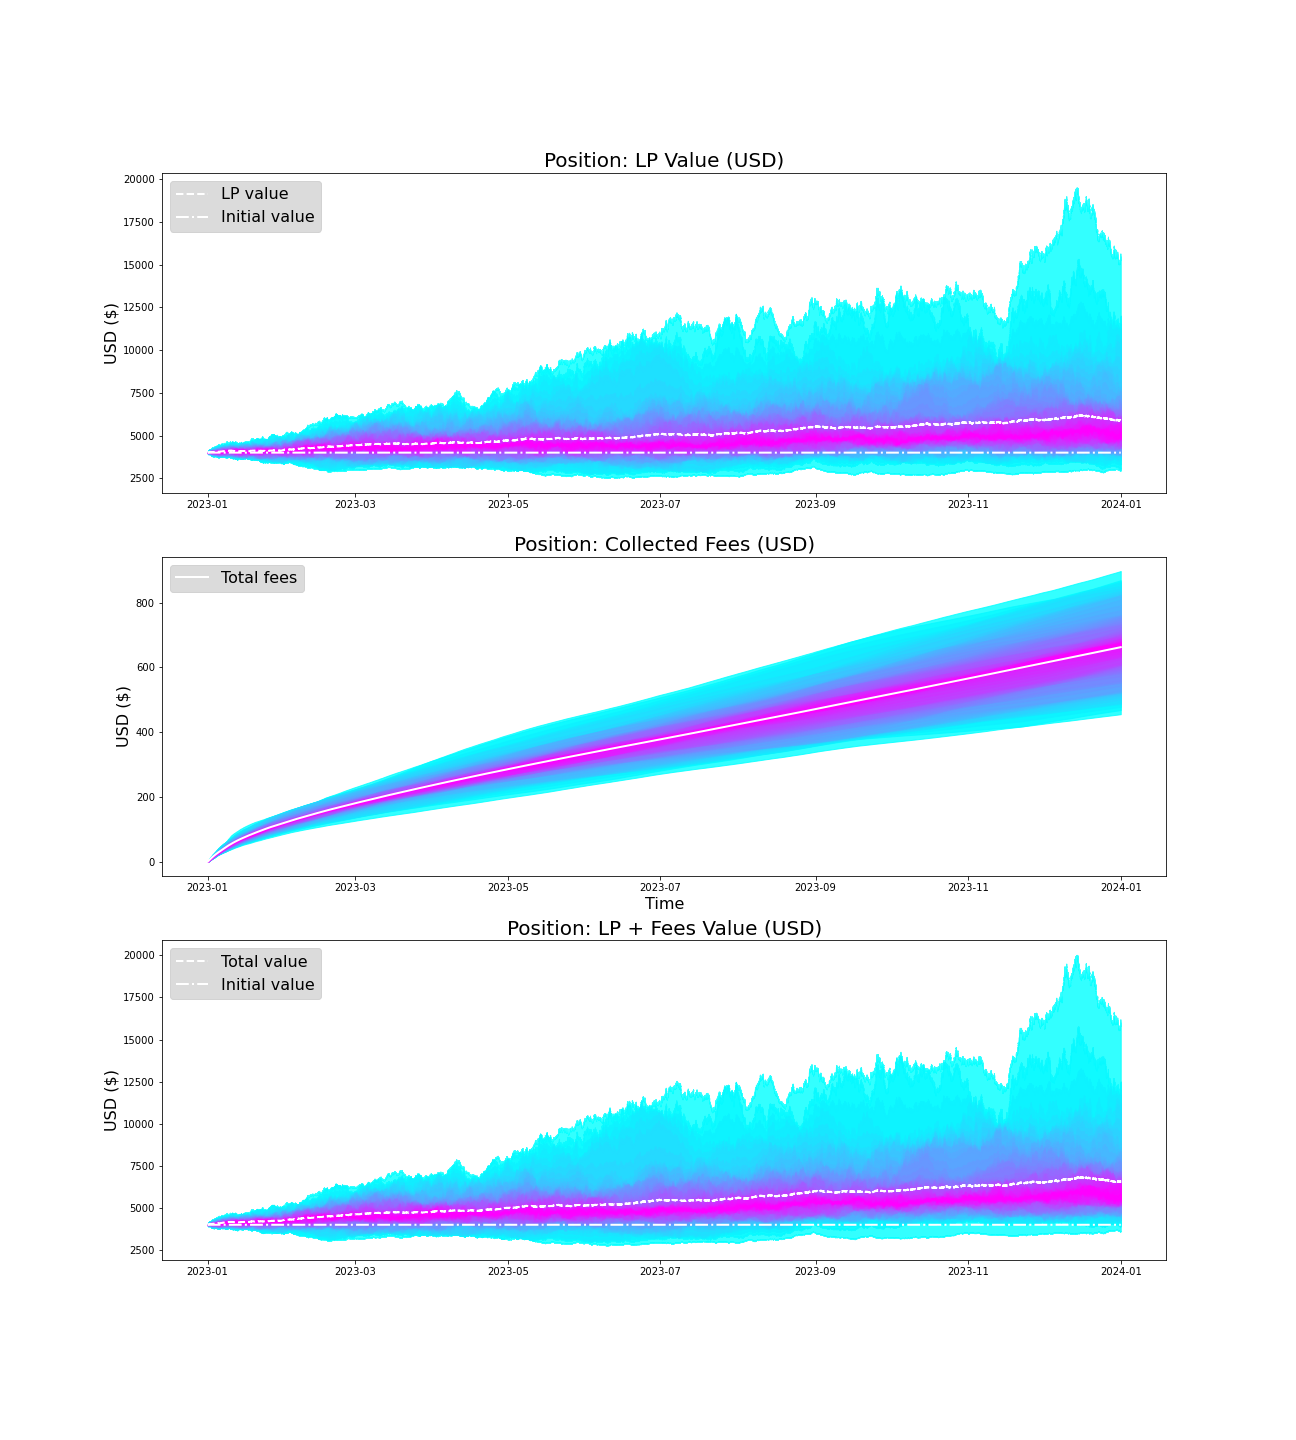
\includegraphics[width=3in]{img/lp_position_values.png}
\caption{Simulation USD values of a LP position with an original value of \$4,000 USD (10,000 SYS and \$2,000 DIA); (TOP) LP USD value of position holdings, where the horizontal line represents initial investment, and dotted line represents the expectation; (MIDDLE) collected fees from position holdings where dotted line represents the expectation; and (BOTTOM) total USD value of position holdings} 
\label{fig:lp_vals}
\end{figure}


\begin{figure}[h!]
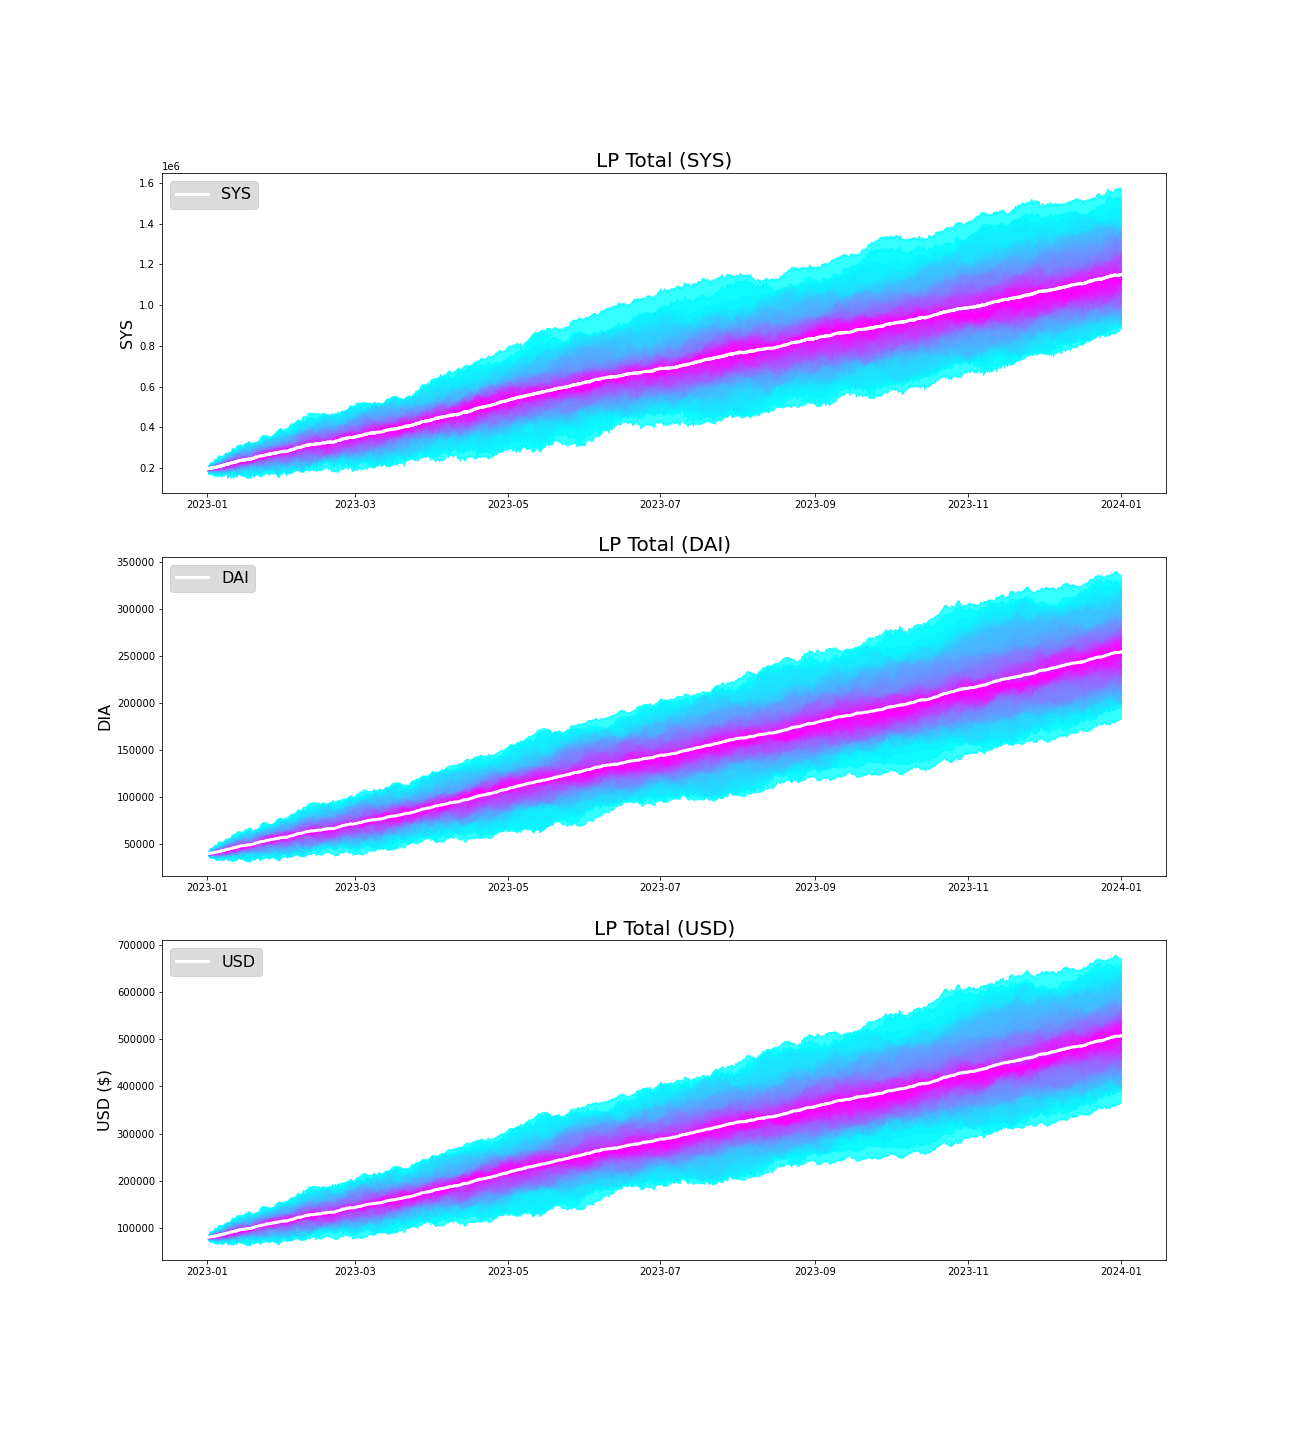
\includegraphics[width=3in]{img/lp_simulation.png}
\caption{Simulated holdings of each asset SYS, DAI and total LP valued in USD within pool. (TOP) LP SYS total; (MIDDLE) LP DAI total; (BOTTOM) LP USD total } 
\label{fig:lp_sims}
\end{figure}


\begin{table}[h!]
\centering
\begin{tabular}{|c|c ||c|c||c|c||c|c| } 
\hline
\multicolumn{2}{|c}{ }  & \multicolumn{2}{c }{ Fees (\%) } & \multicolumn{2}{c}{ Imp Loss (\%)}  & \multicolumn{2}{c|}{ Gain / Loss (\%)}\\
$\mu$ & $\sigma$ & Theo.  & Sim. & Theo.& Sim.& Theo. & Sim. \\
\hline
 \multirow{3}{*}{0.4} & \multirow{3}{*}{0.5} & 4.75  & 4.86 & -4.98 & -4.79 & -0.36  & -0.78 \\
                          &  &  5.15 & 5.28 & -4.98  & -4.13  & 0.04 & 0.20 \\
                          &  &  5.33 & 5.47 & -4.98  & -3.93 & 0.22  & 0.69   \\
\hline
\multirow{ 3}{*}{0.1} & \multirow{3}{*}{0.1} & 3.28  & 3.33 & -0.25 & -0.29 & 3.07  & 2.84 \\
                          &  &  3.09 & 3.13 & -0.25 & -0.22 & 2.88 & 2.78 \\
                          &  &  3.17 & 3.22 & -0.25 & -0.21 & 2.96 & 2.90  \\
\hline
\multirow{ 3}{*}{0.8} & \multirow{3}{*}{0.4} & 5.14  & 5.28 & -9.33 & -9.58 & -4.55 & -6.29\\
                           &  & 4.74  & 4.85 &  -9.33  & -7.33 &   -4.93  &  -4.38  \\
                           &  & 4.78  & 4.90 & -9.33  & -6.88 &  -4.89 & -3.82   \\
\hline
\end{tabular}
\caption{Theoretical versus simulated calculations for expected IL and returns; low liquidity (N = 5,000)}
\label{table:sim_vs_theory1}
\end{table}

\begin{table}[h!]
\centering
\begin{tabular}{|c|c ||c|c||c|c||c|c| } 
\hline
\multicolumn{2}{|c}{ }  & \multicolumn{2}{c }{ Fees (\%) } & \multicolumn{2}{c}{ Imp Loss (\%)}  & \multicolumn{2}{c|}{ Gain / Loss (\%)}\\
$\mu$ & $\sigma$ & Theo.  & Sim. & Theo.& Sim.& Theo. & Sim. \\
\hline
\multirow{3}{*}{0.4} & \multirow{3}{*}{0.5} & 8.82  & 9.22 & -4.98 & -5.79 & 3.78  & 1.34 \\
                          &  &  8.72 & 9.12 &  -4.98 & -6.07  & 3.68 & 1.25 \\
                          &  & 8.49  &  8.86 & -4.98 &  -3.80 & 3.43  &  3.82  \\
\hline
\multirow{ 3}{*}{0.1} & \multirow{3}{*}{0.1} & 5.45  & 5.60 &  -0.25 & -0.23 & 5.33 & 5.08 \\
                          &  & 5.41 & 5.56 &  -0.25  & -0.19 & 5.29  & 5.12  \\
                          &  & 5.22  & 5.36 & -0.25  & -0.27 &  5.09 & 4.80   \\
\hline
\multirow{ 3}{*}{0.8} & \multirow{3}{*}{0.4} & 8.52 &  8.89 &  -9.33 & -8.75 & -1.27 & -3.22 \\
                         &  & 8.40  & 8.76 & -9.33  & -7.81 &  -1.39  &  -2.06  \\
                         &  & 8.67  & 9.06 & -9.33  & -7.84 & -1.12  &  -1.99   \\
\hline
\end{tabular}
\caption{Theoretical versus simulated calculations for expected IL and returns; high liquidity (N = 25,000)}
\label{table:sim_vs_theory2}
\end{table}


\begin{table}[h!]
\centering
\begin{tabular}{|c||c|c||c|c|} 
\hline
 & \multicolumn{2}{c}{ High Liquidity } & \multicolumn{2}{c|}{ Low Liquidity } \\
 & volatility ($\sigma$) & drift ($\mu$) & volatility ($\sigma$) & drift ($\mu$) \\
\hline
Small & 2 & 2 & 1 & 1 \\
Medium & $0^{+}$ & $0^{+}$ & 0 & 0 \\
Large & -1 & -1 & -2 & -2 \\
\hline
\end{tabular}
\caption{General guideline (ranked by potential profitability) DEXs can apply to their LP management strategy for asset holdings $x$ and $y$, where $\mu$ and $\sigma$ represent drift and volatility of historical asset prices (ie, $p_{k} = \frac{y_{k}}{x_{k}}$); -2 $\rightarrow$ potential for loss, 0 -> neutral, and 2 $\rightarrow$ potential for gain. }
\label{table:profitability_guideline}
\end{table}

\section{Summary}
\label{section:summary}

In this discussion we perform an analytical and numerical survey of IL for Uniswap v2. If we assume prices behave as a GBM process, we show that IL is exactly computable in closed form (\ref{eqn:exp_imp_loss}), and that its computation can be extended to calculate expected returns with compounding fees (\ref{eqn:exp_returns_with_fees}). 

We also set up simulations and show that the experimental outcomes also align to the theoretical calculations. The simulator used in this work can be easily extended to include various edge cases to understand risk tolerances aprior to execution which is openly available on Syscoin's Github repos \cite{DAOSim23}, and is the subject of future work.

The theory presented here is very useful for LP managers as we have shown that portfolio risk due to IL can be pre-determined through a relatively straight forward back-of-the-envelope calculation, given an asset's historical price drift and volatility. Also, if we have some idea on historical returns due to fees, we have shown that overall expected LP returns can also be estimated in a similar straight forward way. To summarize, we have provided a broad profitability guideline for business managers to follow in Table \ref{table:profitability_guideline}. The fee model that we used is relatively straight forward, and with some additional exploration, the expected returns formula can be updated to better cater to the various forms of LP behavior. 

Finally, if long-term profitability is the overall intended goal, these calculations will help remove a lot of the guess work when managing LP risk.  

\appendices

\section{Geometric Brownian Motion}
\label{sec:gbm}

Brownian motion (or Wiener Process) is a type of non-stationary stochastic process used to model natural phenomena studied in the Applied Sciences, and is represented as the following distribution:
\begin{equation}\label{eqn:bm}
  W_{t} \sim N(0,t), 
\end{equation}
where $t$ represents some time period. A well-known risky asset model for prices, $S_{t}$, are represented by the following differential equation:
\begin{equation}\label{eqn:asset_model}
  dS_{t} = \mu S_{t}dt + \sigma S_{t} dW_{t},
\end{equation}
where $\mu$ represents the drift and $\sigma$ represents the volatility of the asset. The solution to the asset model of (\ref{eqn:asset_model}) is given by:
\begin{equation}\label{eqn:gbm}
  S_{t} = S_{0} e^{(\mu - \frac{\sigma^2}{2})t  + \sigma W_{t}},
\end{equation}
which is known as Geometric Brownian Motion (GBM). The idea of using (\ref{eqn:gbm}) to model stock prices was first discovered by Bachelier \cite{Bac1900} and popularized by Samuelson in \cite{Sam65}; details on the derivation of this solution can be found in Chapter 1 of \cite{Pri23}.

\section{MGF of Brownian Motion}
\label{sec:exp_brownian_motion}

The moment generating function (MGF), $M(a)$, for a random variable X is $E\{e^{aX}\}$. Thus, the MGF of a normal random variable is given by:
\begin{eqnarray*}\label{eqn:mgf_normal}
M(a) &=& E\{e^{aX}\}\\ 
           &=& \int_{-\infty}^{\infty}e^{ax}f(x)dx \\
           &=& e^{a\mu + \frac{1}{2}a^2\sigma^2},
\end{eqnarray*}
where $X \sim N(\mu, \sigma^2)$. Since a standard Brownian motion process, $W_{t}$, is also normally distributed where $W_{t} \sim N(0,t)$, we have:

\begin{equation}\label{eqn:mgf_bm}
  E\{e^{aW_{t}}\} = e^{\frac{1}{2}a^2t}.
\end{equation}


\section{Expected Impermanent Loss Derivation}
\label{sec:exp_imp_loss_derv}

Under the assumption of GBM, equations (\ref{eqn:initial_lp_value}) and (\ref{eqn:held_lp_value}) can be represented as:

\begin{equation}\label{eqn:initial_lp_value_gbm}
V_{t} = 2L\sqrt{P_{0} e^{(\mu - \frac{\sigma^2}{2})t + \sigma W_{t} } },
\end{equation}
and  
\begin{equation}\label{eqn:held_lp_value_gbm}
V_{H,t} = 2L\sqrt{P_{0}} ( 1 + e^{(\mu - \frac{\sigma^2}{2})t + \sigma W_{t} } ).
\end{equation}
Using the MGF of standard Brownian motion from (\ref{eqn:mgf_bm}) and (\ref{eqn:initial_lp_value_gbm}), we calculate $E\{V\}$:

\begin{eqnarray*}\label{eqn:derivation_exp_v0}
E\{V\} &=& E\{2L \sqrt{P_{0}} e^{(\frac{\mu}{2} - \frac{\sigma^2}{4})t } e^{   \frac{1}{2}\sigma W_{t} } \} \\ 
           &=& 2L \sqrt{P_{0}} e^{(\frac{\mu}{2} - \frac{\sigma^2}{4})t } E\{e^{ \frac{1}{2}\sigma W_{t} }\} \\
           &=& 2L \sqrt{P_{0}} e^{(\frac{\mu}{2} - \frac{\sigma^2}{4})t } e^{\frac{\sigma^2 t}{8}} \\
           &=&  2L \sqrt{P_{0}}e^{( \frac{\mu}{2} - \frac{\sigma^2}{8})}.
\end{eqnarray*}
Likewise, using the same MGF of standard Brownian motion from (\ref{eqn:mgf_bm}) and (\ref{eqn:held_lp_value_gbm}), we calculate $E\{V_{H}\}$: 
\begin{eqnarray*}\label{eqn:derivation_exp_vH}
E\{V_{H}\} &=& E\{L \sqrt{P_{0}}(1 + e^{(\mu - \frac{\sigma^2}{2})t + \sigma W_{t} })\} \\
		   &=& L \sqrt{P_{0}}(1 + E\{ e^{(\mu - \frac{\sigma^2}{2})t + \sigma W_{t} }  \}) \\
		   &=& L \sqrt{P_{0}}(1 + e^{(\mu - \frac{\sigma^2}{2})t} E\{e^{\sigma W_{t}}\} ) \\
		   &=& L \sqrt{P_{0}}(1 + e^{(\mu - \frac{\sigma^2}{2})t} e^{\frac{1}{2} \sigma^2 t} \\
		   &=& L \sqrt{P_{0}}(1 + e^{\mu t} ).
\end{eqnarray*}
Therefore using the the identity $\cosh(x) = \frac{1 + e^{2x}}{2 e^x}$, and our definition of IL outlined in (\ref{eqn:imp_loss})  we have:
\begin{eqnarray*}\label{eqn:derivation_exp_IL}
E\{IL\} &=& \frac{E\{V_{0}\} - E\{V_{H}\}}{E\{V_{H}\}} \\
		&=& \frac{2L \sqrt{P_{0}}e^{( \frac{\mu}{2} - \frac{\sigma^2}{8})} }{L \sqrt{P_{0}}(1 + e^{\mu t} )}\\
		&=& \frac{2e^{( \frac{\mu}{2} - \frac{\sigma^2}{8})}}{1 + e^{\mu t}} - 1\\
		&=& \frac{e^{-\frac{\sigma^2 t}{8}}}{ cosh(\frac{\mu t}{2})} - 1.
\end{eqnarray*}


\section{Solve LP Swap Deltas}
\label{sec:lp_swap_deltas}
Here we address the problem of updating asset balances (ie, $x_{k}$,$y_{k}$) upon each price change $\Delta p_{k}$, where $\{p_{k}\}_{0}^{N}$ is a simulated GBM process representing the prices of our asset (valued in USD) over time sample $k$. Price change, $\Delta p_{k}$, in a liquidity pool are determined as:

\begin{eqnarray*}\label{eqn:deltap1}
\Delta p_{k} &=& \frac{y_{k}}{x_{k}} - \frac{y_{k-1}}{x_{k-1}} \\
			 &=& \frac{\Delta y_{k} + y_{k-1}}{\Delta x_{k} + x_{k-1}} - \frac{y_{k-1}}{x_{k-1}},
\end{eqnarray*}
and asset trade price is determined as: 
\begin{equation}\label{eqn:deltap2}
  p_{k} = \frac{\Delta y_{k}}{\Delta x_{k}}.
\end{equation}
Thus, given the above equations, we derive the following system of non-linear equations:
\begin{eqnarray}\label{eqn:non_linear_system}
\frac{x_{k-1} \Delta y_{k} - \Delta x_{k} y_{k-1}}{x_{k-1}^2 + x_{k-1} \Delta x_{k}} - \Delta p_{k} &=& 0 \\
\frac{\Delta y_{k}}{\Delta x_{k}} - p_{k} &=& 0.
\end{eqnarray}
Since we have the previous balances $y_{k-1}$, $x_{k-1}$, price change $\Delta p_{k}$, and the current price $p_{k}$ from our simulated GBM, we can solve for the swap balances $\Delta x_{k}$ and $\Delta y_{k}$ under the constraints $\Delta y_{k} > 0$ and $\Delta x_{k} > 0$ for every $k$. To achieve this, we used the \verb|optimize.fsolve| function from \verb|scipy| package in python. 


\begin{thebibliography}{00}

\bibitem{Pin19a} Pintail, \textit{Uniswap: A Good Deal for Liquidity Providers?}, Jan. 2019. Accessed on: Dec 2022.  [Online]. Available:  https://pintail.medium.com/uniswap-a-good-deal-for-liquidity-providers-104c0b6816f2

\bibitem{Pin19b} Pintail, \textit{Understanding Uniswap Returns}, Feb. 2019. Accessed on: Dec 2022.  [Online]. Available:  hhttps://pintail.medium.com/understanding-uniswap-returns-cc593f3499ef

\bibitem{Doge22} C. Doge, I. Moore, R. Arbour, and J. Sidhu, \textit{DOASYS, Smart DAO Protocol for Decentralized Finance}, Syscoin Github repos, Oct. 2022, Accessed on: Mar 2023.  [Online]. Available: https://github.com/syscoin/daosys/blob/main/latex/whitepaper/article.pdf

\bibitem{Pet21} P. Erins, \textit{How to calculate Impermanent Loss: full derivation}, Jun. 2021. Accessed on: Dec 2022.  [Online]. Available:  https://medium.com/auditless/how-to-calculate-impermanent-loss-full-derivation-803e8b2497b7

\bibitem{Aig21} A. Aigner and G. Dhaliwal, \textit{UNISWAP: Impermanent Loss and Risk Profile of a Liquidity Provider}, Jun. 2021. Accessed on: Dec 2022.  [Online]. Available:  https://arxiv.org/pdf/2106.14404.pdf

\bibitem{Gui21} G. Lambert, \textit{Calculating the Expected Value of the Impermanent Loss in Uniswap}, Oct. 2021. Accessed on: Dec 2022.  [Online]. Available:  https://lambert-guillaume.medium.com/an-analysis-of-the-expected-value-of-the-impermanent-loss-in-uniswap-bfbfebbefed2

\bibitem{Dan22} Danr, \textit{Expected Impermanent Loss in Uniswap V2 \& V3}, Mar. 2022. Accessed on: Dec 2022.  [Online]. Available:  https://medium.com/gammaswap-labs/expected-impermanent-loss-in-uniswap-v2-v3-7fb81033bd81

\bibitem{Dec21} Danr, \textit{Total Returns and Impermanent Loss in Uniswap V2}, Dec. 2021. Accessed on: Dec 2022.  [Online]. Available:  https://medium.com/gammaswap-labs/total-returns-and-impermanent-loss-in-uniswap-v2-9f3d5b6ebc89

\bibitem{Pri23} N. Privault, \textit{Notes on Financial Risk \& Analytics}, Jan 2023, Accessed on: Feb 2023.  [Online]. Available:  https://personal.ntu.edu.sg/nprivault/MH8331/financial\_risk\_analytics.pdf


\bibitem{Uni19} Uniswap Blog, \textit{A short history of Uniswap}, Sept. 2019. Accessed on: Sept 2022.  [Online]. Available:  https://uniswap.org/blog/uniswap-history

\bibitem{Moo22A} I.C. Moore,  \textit{Masternode Yield Farming as a DAOSYS Usecase: Part 1}, Medium Article, Aug. 2022. Accessed on: Sept 2022.  [Online]. https://icmoore.medium.com/masternode-yield-farming-as-a-daosys-usecase-part-1-8485ab7ba721

\bibitem{Moo22B} I.C. Moore,  \textit{Masternode Yield Farming as a DAOSYS Usecase: Part 2}, Medium Article, Aug. 2022. Accessed on: Sept 2022.  [Online]. https://icmoore.medium.com/masternode-yield-farming-as-a-daosys-usecase-part-2-8906d0a11c27

\bibitem{DAOSim22} I.C. Moore, \textit{Simulation: Masternode Yield Farming}, Syscoin Github repos, Accessed on: Apr 2021.  [Online]. Available: https://github.com/syscoin/daosys/tree/main/notebooks/simulation

\bibitem{DAOSim23} I.C. Moore , \textit{Simulation: LP Activity using GBM}, Syscoin Github repos, Accessed on: Apr 2021.  [Online]. Available: https://github.com/syscoin/daosys/tree/main/notebooks/research/impermanent\_loss


\bibitem{ROL22} Syscoin News, \textit{Introducing Rollux, Syscoin's Rollup Suite Ready to Take Market by Storm}, Syscoin, Jun. 2022. Accessed on: Sept 2022.  [Online]. Available: https://syscoin.org/news/introducing-rollux-syscoins-rollup-suite-ready-to-take-market-by-storm

\bibitem{Sig21a} J. Sidhu, \textit{A Design For An Efficient Coordinated Financial Computing Platform}, Feb 2021, Accessed on: Sep 2021.  [Online]. Available:  https://jsidhu.medium.com/a-design-for-an-efficient-coordinated-financial-computing-platform-ab27e8a825a0

\bibitem{Sig21b} J. Sidhu and I.C. Moore, \textit{Syscoin 4: A Peer-to-Peer Electronic Cash System Built For Decentralized
Web 3.0 Business Applications}, Syscoin Platform, Dec. 2021. Accessed on: Sept 2022. [Online]. Available: https://syscoin.org/$syscoin4\_whitepaper.pdf$

\bibitem{Sam65} P. Samuelson, \textit{Rational Theory of Warrant Pricing}, Industrial Management Review (pre-1986), Cambridge Vol. 6, Iss. 2, (Spring 1965): 13.

\bibitem{Bac1900} L. Bachelier, \textit{Théorie de la spéculation},  Annales scientifiques de l'École Normale Supérieure, Série 3, Tome 17 (1900), pp. 21-86.


\end{thebibliography}


\EOD

\end{document}
